\section{Bestimmung Reibungskoeffizient}\label{anhang:herleitung:reibungskoeffizient}
Um den Reibungskoeffizienten $c_R$ zu bestimmen, wird ein Versuchsaufbau in Form einer Rampe benötigt, wobei eine
theoretische Reibung auf einer perfekt glatten Oberfläche der Rampe von $0$ angenommen wird.

\begin{figure}[h!]
    \begin{center}
        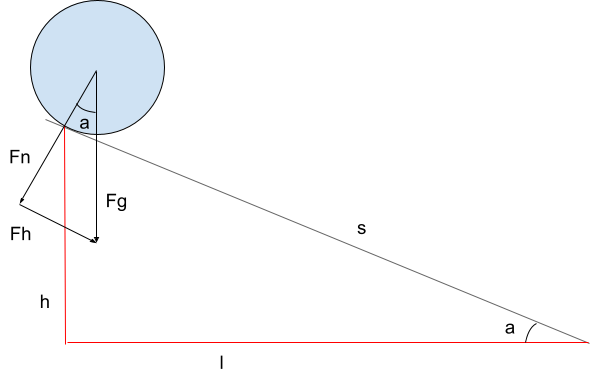
\includegraphics[width=0.5\linewidth]{../common/07_appendix/resources/00_reibungskoeffizient_rampe.png}
    \end{center}
    \caption{Modell zur Berechnung der Startgeschwindigkeit auf dem Tisch}
    \label{fig:modell_berechnung_startgeschwindigkeit}
\end{figure}

In Abbildung \ref{fig:modell_berechnung_startgeschwindigkeit} werden die wirkenden Kräfte und ihr Einfluss veranschaulicht.
Es gelten die nachfolgenden Beziehungen.

\begin{align}
    g = 9.81 \frac{m}{s^2}\\
    \alpha = \arctan(\frac{h}{l})\\
    F_G = m \cdot g\\
    F_N = \cos(\alpha) * F_G\\
    F_H = \sin(\alpha) * F_G\\
    s = \sqrt{l^2 + h^2}\\
\end{align}

Während die Kugel die Rampe herunterrollt, wird die Formel der gleichmässig beschleunigten Bewegung verwendet.
Die Kugel wird auf der Rampe platziert und losgelassen. Das bedeutet, dass sie keine Initialgeschwindigkeit hat.
Relevant ist am Ende die zurückgelegte Strecke wie auch die benötigte Zeit.
\begin{align}
    s(t) = s = \frac{1}{2} \cdot a \cdot t^2 + v_0 \cdot t + s_0\\
    v_0 = 0\\
    s_0 = 0\\
    s(t) = s = \frac{1}{2} \cdot a \cdot t^2\\
    F_H = m \cdot a\\
    a = \frac{F_H}{m}\\
    \frac{1}{2} \cdot \frac{F_H}{m} \cdot t^2 - s = 0
\end{align}

Der Zeitpunkt, wo die Kugel das Ende der Rampe erreicht, kann mithilfe der allgemeinen Lösungsformel für quadratische Gleichungen nach $t$ gelöst werden \cite{wiki.mitternachtsformel:1}:
\begin{align}
    t_{1,2} = \frac{-b \pm \sqrt{b^2 - 4ac}}{2a}\\
    a = \frac{1}{2} \cdot \frac{F_H}{m}\\
    b = 0\\
    c = -s\\
    t_{1,2} = \frac{\pm \sqrt{-4ac}}{2a}\\
\end{align}

Es wird nur die positive Lösung in Betracht gezogen.

Die Geschwindigkeit der Kugel am Ende der Rampe ist somit:
\begin{align}
    v(t) = a \cdot t + v_0\\
    v_0 = 0\\
    v(t) = \frac{F_H}{m} \cdot t
\end{align}

TODO: Kollision mit Tisch?

Ab diesem Zeitpunkt wird angenommen, dass die Kugel auf dem Tisch rollt und nur noch von der Rollreibung zwischen Kugel und Tisch abgebremst wird.
Es muss die von der Kugel bis zum Stillstand zurückgelegte Strecke $s$ gemessen werden.
Weiterhin gelten die Beziehungen in Abbildung \ref{fig:modell_reibungskoeffizient}.

\begin{figure}[h!]
    \begin{center}
        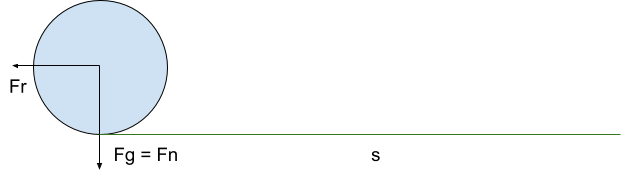
\includegraphics[width=0.5\linewidth]{../common/07_appendix/resources/01_reibungskoeffizient_tisch.png}
    \end{center}
    \caption{Modell zur Berechnung des Reibungskoeffizienten}
    \label{fig:modell_reibungskoeffizient}
\end{figure}

Anschliessend kann die Beschleunigung berechnet werden:
\begin{align}
    s(t) = s = \frac{1}{2} \cdot a \cdot t^2 + v_0 \cdot t + s_0\\
    s_0 = 0\\
    v_0 = v(t_R)\\
    \frac{1}{2} \cdot a \cdot t^2 + v_0 \cdot t - s = 0\\
    v(t) = 0 = a \cdot t + v_0\\
    a \cdot t = -v_0\\
    t = \frac{-v_0}{a}\\
    \frac{1}{2} \cdot a \cdot (\frac{-v_0}{a})^2 + v_0 \cdot \frac{-v_0}{a} - s = 0\\
    \frac{1}{2} \cdot a \cdot \frac{(-v_0)^2}{a^2} + v_0 \cdot \frac{-v_0}{a} - s = 0\\
    \frac{1}{2} \cdot \frac{(-v_0)^2}{a} + v_0 \cdot \frac{-v_0}{a} - s = 0\\
    \frac{1}{2} \cdot (-v_0)^2 \cdot \frac{1}{a} + v_0 \cdot (-v_0) \cdot \frac{1}{a} - s = 0\\
    \frac{1}{a} \cdot (\frac{1}{2} \cdot (-v_0)^2 + v_0 \cdot (-v_0)) - s = 0\\
    \frac{1}{2} \cdot (-v_0)^2 + v_0 \cdot (-v_0) = s \cdot a\\
    a = \frac{\frac{1}{2} \cdot (-v_0)^2 + v_0 \cdot (-v_0)}{s}
\end{align}

Mit der Beschleunigung kann nun der Rollwiderstandskoeffizient berechnet werden.
Da die Kugel auf dem Tisch liegt, ist die Normalenkraft $F_N$ gleich der Gewichtskraft $F_G$.

\begin{align}
    F_R = c_R \cdot F_N\\
    F_R = m \cdot a\\
    F_N = F_G\\
    F_G = m \cdot g\\
    m \cdot a = c_R \cdot m \cdot g\\
    c_R = \frac{m \cdot a}{m \cdot g}\\
    c_R = \frac{a}{g}
\end{align}

